\renewcommand{\thetheorem}{5.\arabic{theorem}}
\setcounter{theorem}{0}
\setcounter{chapter}{4}

\chapter{Fields (Körper)}

Before we can solve systems of linear equations or define abstract vector spaces, we must answer a more fundamental question: \textit{Where do our numbers come from?} 

In linear algebra, we do not restrict ourselves to the real numbers. We can perform our calculations over any algebraic structure where addition, subtraction, multiplication, and division behave exactly as we expect them to. Such a structure is called a \textbf{field} (in German: \textit{Körper}).

\subsection{The Field Axioms}

To ensure that an algebraic structure behaves nicely, it must satisfy nine rigid rules. These are the Field Axioms.

\begin{definition}[Field]
A \textit{field} is a tuple $(K, +, \cdot, 0, 1)$ consisting of a set $K$ equipped with two binary operations:
\begin{align*}
&+: K \times K \rightarrow K, \quad (x, y) \mapsto x + y \quad \text{(Addition)} \\
&\cdot: K \times K \rightarrow K, \quad (x, y) \mapsto x \cdot y \quad \text{(Multiplication)}
\end{align*}
and two distinguished, unique elements $0, 1 \in K$, such that the following nine axioms hold:

\noindent
\textbf{Axioms of Addition:}
\begin{enumerate}[label=(K\arabic*), leftmargin=3.5em]
    \item $\forall x, y, z \in K: x + (y + z) = (x + y) + z$ \hfill \textit{(Associativity of Addition)}
    \item $\forall x, y \in K: x + y = y + x$ \hfill \textit{(Commutativity of Addition)}
    \item $\forall x \in K: 0 + x = x$ \hfill \textit{(Neutral Element of Addition)}
    \item $\forall x \in K, \exists x' \in K: x + x' = 0$ \hfill \textit{(Inverse Element of Addition)}
\end{enumerate}

\noindent
\textbf{Axioms of Multiplication:}
\begin{enumerate}[label=(K\arabic*), start=5, leftmargin=3.5em]
    \item $\forall x, y, z \in K: x \cdot (y \cdot z) = (x \cdot y) \cdot z$ \hfill \textit{(Associativity of Multiplication)}
    \item $\forall x \in K: 1 \cdot x = x$ \hfill \textit{(Neutral Element of Multiplication)}
    \item $\forall x \in K \setminus \{0\}, \exists x' \in K: x' \cdot x = 1$ \hfill \textit{(Inverse Element of Multiplication)}
\end{enumerate}

\noindent
\textbf{Compatibility and Non-Triviality:}
\begin{enumerate}[label=(K\arabic*), start=8, leftmargin=3.5em]
    \item $\forall x, y, z \in K: x \cdot (y + z) = x \cdot y + x \cdot z$ \hfill \textit{(Distributivity)}
    \item $1 \ne 0$ \hfill \textit{(The field has at least two elements)}
\end{enumerate}
\end{definition}

\begin{remark}[Notation]
We typically denote the additive inverse $x'$ from (K4) as $-x$, allowing us to define subtraction: $x - y := x + (-y)$. 
Similarly, we denote the multiplicative inverse $x'$ from (K7) as $x^{-1}$ or $\frac{1}{x}$, allowing us to define division by non-zero elements: $x / y := x \cdot y^{-1}$.
\end{remark}

\subsection{Infinite Fields}

The most familiar fields are infinite. They form the backbone of calculus and classical geometry.

\begin{example}[Familiar Infinite Fields]
\begin{itemize}
    \item $\mathbb{Q}$: The rational numbers (fractions). This is the smallest field containing the integers.
    \item $\mathbb{R}$: The real numbers.
    \item $\mathbb{C}$: The complex numbers, where we introduce $i^2 = -1$.
\end{itemize}
\end{example}

\begin{importantremark}
The integers $\mathbb{Z} = \{\dots, -2, -1, 0, 1, 2, \dots\}$ do \textbf{not} form a field! While they satisfy addition and multiplication axioms perfectly, they completely fail (K7). For instance, there is no integer $x'$ such that $2 \cdot x' = 1$. You cannot divide freely within $\mathbb{Z}$.
\end{importantremark}

\subsection{Finite Fields and Modular Arithmetic}

A field does not have to be an infinite, continuous line of numbers. If we change our definitions of "addition" and "multiplication", we can create perfectly valid fields that contain only a finite number of elements.

The secret to building a finite field is \textit{modular arithmetic} (often called "clock arithmetic"). Instead of numbers growing infinitely on a number line, they wrap around a circle.

\begin{center}
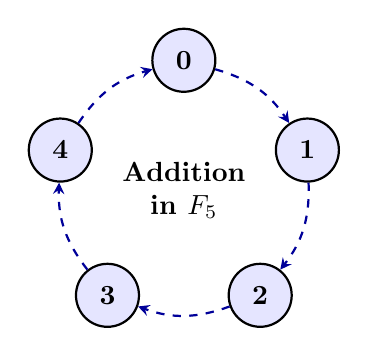
\begin{tikzpicture}[scale=1.1,
    node distance=2cm,
    box/.style={circle, draw, thick, fill=blue!10, minimum size=8mm, align=center},
    arrow/.style={->, thick, >=stealth, dashed, draw=blue!60!black}
]
    % Draw a clock for F_5
    \foreach \i/\label in {90/0, 18/1, -54/2, -126/3, -198/4} {
        \node[box] (\label) at (\i:1.5) {\textbf{\label}};
    }
    
    \draw[arrow, bend left=20] (0) to (1);
    \draw[arrow, bend left=20] (1) to (2);
    \draw[arrow, bend left=20] (2) to (3);
    \draw[arrow, bend left=20] (3) to (4);
    \draw[arrow, bend left=20] (4) to (0);
    
    % FIXED NODE ALIGNMENT HERE
    \node[align=center] at (0,0) {\textbf{Addition} \\ \textbf{in $\mathbb{F}_5$}};
\end{tikzpicture}
\end{center}

\begin{definition}[The Field $\mathbb{F}_p$]
Let $p$ be a prime number. The set of integers modulo $p$, denoted as $\mathbb{F}_p$ (or sometimes $\mathbb{Z}/p\mathbb{Z}$), contains exactly $p$ elements:
\[
\mathbb{F}_p = \{0, 1, 2, \dots, p-1\}
\]
Addition and multiplication are performed exactly as regular integers, but if the result exceeds $p-1$, we divide by $p$ and keep only the \textbf{remainder}.
\end{definition}

\begin{theorem}
$\mathbb{F}_p$ is a field if and only if $p$ is a prime number.
\end{theorem}

Why must $p$ be prime? Consider what happens if we try to build a field modulo $4$ (which is not prime). In modulo $4$, we have $2 \cdot 2 = 4 \equiv 0 \pmod 4$. We multiplied two non-zero numbers and got zero! In a true field, this is algebraically impossible, because it destroys the ability to divide (axiom K7). Prime numbers beautifully prevent this "zero divisor" problem.

\begin{example}[The Smallest Field: $\mathbb{F}_2$]
The absolute smallest field mathematically possible contains only two elements: $\{0, 1\}$. This is the field of Boolean logic, heavily used in computer science and cryptography. Operations are done modulo $2$:
\[
\begin{array}{c|cc}
+ & 0 & 1 \\
\hline
0 & 0 & 1 \\
1 & 1 & 0
\end{array}
\qquad\qquad\qquad
\begin{array}{c|cc}
\cdot & 0 & 1 \\
\hline
0 & 0 & 0 \\
1 & 0 & 1
\end{array}
\]
Notice the fascinating property of $\mathbb{F}_2$: $1 + 1 = 0$. In this field, every element is its own additive inverse! Subtraction and addition are literally the same operation.
\end{example}

\begin{example}[Calculations in $\mathbb{F}_5$]
Let us explore $\mathbb{F}_5 = \{0, 1, 2, 3, 4\}$.
\begin{itemize}
    \item \textbf{Addition:} $3 + 4 = 7$. But $7 \div 5 = 1$ with a remainder of $2$. So, $3 + 4 = 2$ in $\mathbb{F}_5$.
    \item \textbf{Additive Inverses \textbf{(K4)}:} What is $-2$? We need a number that adds to $2$ to yield $0$. Since $2 + 3 = 5 \equiv 0$, we know that $-2 = 3$.
    \item \textbf{Multiplicative Inverses \textbf{(K7)}:} What is the inverse of $3$ (i.e., $\frac{1}{3}$)? We need a number $x$ such that $3 \cdot x = 1$. Let's test the options: $3 \cdot 2 = 6 \equiv 1$. Therefore, $3^{-1} = 2$.
\end{itemize}
\end{example}

\subsection{Proving Basic Properties from the Axioms}

The power of an axiomatic definition is that if we can prove a theorem using \textit{only} axioms \textbf{(K1)} through \textbf{(K9)}, that theorem is universally true for \textbf{every field in existence}—whether it is the infinite space of real numbers $\mathbb{R}$, or the tiny binary world of $\mathbb{F}_2$.

Let us prove two seemingly "obvious" facts that actually require careful algebraic footwork to justify.

\begin{lemma}[Multiplication by Zero]
For any element $x$ in a field $K$, we have $0 \cdot x = 0$.
\end{lemma}

\begin{proof}
Let $x \in K$. By the neutral property of zero \textbf{(K3)}, we know that $0 = 0 + 0$. 
Let us multiply both sides of this equation by $x$:
\[
(0 + 0) \cdot x = 0 \cdot x
\]
By the distributivity axiom \textbf{(K8)}, we can expand the left side:
\[
0 \cdot x + 0 \cdot x = 0 \cdot x
\]
Now, by the additive inverse axiom \textbf{(K4)}, the element $(0 \cdot x)$ must have an inverse, $-(0 \cdot x)$. We add this inverse to both sides of our equation:
\[
\big(0 \cdot x + 0 \cdot x\big) + \big(-(0 \cdot x)\big) = 0 \cdot x + \big(-(0 \cdot x)\big)
\]
Using associativity of addition \textbf{(K1)}, we regroup the left side:
\[
0 \cdot x + \Big(0 \cdot x + \big(-(0 \cdot x)\big)\Big) = 0
\]
\[
0 \cdot x + 0 = 0
\]
Finally, applying \textbf{(K3)} once more, we drop the $+ 0$ to conclude:
\[
0 \cdot x = 0
\]
\end{proof}

\begin{lemma}[Zero Divisors do not exist]
Let $a, b \in K$. If $a \cdot b = 0$, then either $a = 0$ or $b = 0$.
\end{lemma}

\begin{proof}
Assume $a \cdot b = 0$. We want to show that if $a \ne 0$, then $b$ must be exactly $0$.

Suppose $a \ne 0$. Because $a$ is a non-zero element in a field, axiom \textbf{(K7)} guarantees that it has a multiplicative inverse, $a^{-1}$. 
Let us multiply both sides of our equation $a \cdot b = 0$ by this inverse:
\[
a^{-1} \cdot (a \cdot b) = a^{-1} \cdot 0
\]
From our previous lemma, we know that any element multiplied by $0$ is $0$, so the right side is $0$:
\[
a^{-1} \cdot (a \cdot b) = 0
\]
By associativity of multiplication \textbf{(K5)}, we regroup the left side:
\[
(a^{-1} \cdot a) \cdot b = 0
\]
By the definition of the inverse \textbf{(K7)}, $a^{-1} \cdot a = 1$:
\[
1 \cdot b = 0
\]
Finally, by the neutral element of multiplication \textbf{(K6)}, $1 \cdot b = b$. Thus:
\[
b = 0
\]
We have proven that if the product is zero and $a$ is not zero, $b$ is forced to be zero.
\end{proof}
